\documentclass[14pt]{beamer}

\usetheme{simple}

\usepackage[utf8]{inputenc}
\usepackage[light,sfdefault]{roboto}
\usepackage{color}
% https://tex.stackexchange.com/questions/23711/strikethrough-text
\usepackage{soul}
\usepackage{tikz}
\usepackage{subcaption}
\usepackage{xcolor}
\usepackage[%
  font=normalsize,
  labelfont=normalsize,
  justification=centering
]{caption}

\definecolor{MPIgreen}{RGB}{66,135,59}
\usetikzlibrary{arrows.new}
\tikzset{arrow/.style={-latex new,arrow head=0.25cm}}

\title{A Point Set Generation Network for 3D Object Reconstruction from a Single Image \cite{Fan:2016}}
\author{David Stutz}
\date{June 1-2, 2017}

\begin{document}
  \begin{frame}[plain]
    \titlepage
  \end{frame}

  \begin{frame}
    \frametitle{Motivation}
    
    Addressed problem: 3D reconstruction from a single image.
    \vskip 1em
    
    PointNet \cite{GarciaGarcia:2016}: deep learning on point sets.
    \vskip 1em
    
    Underlying motivation:
    \begin{itemize}
      \item How to learn how to generate shapes, i.e. point sets?
    \end{itemize}
  \end{frame}
  
  \begin{frame}
    \frametitle{Recap: PointNet}
    
    \begin{figure}
      \hspace*{-0.5cm}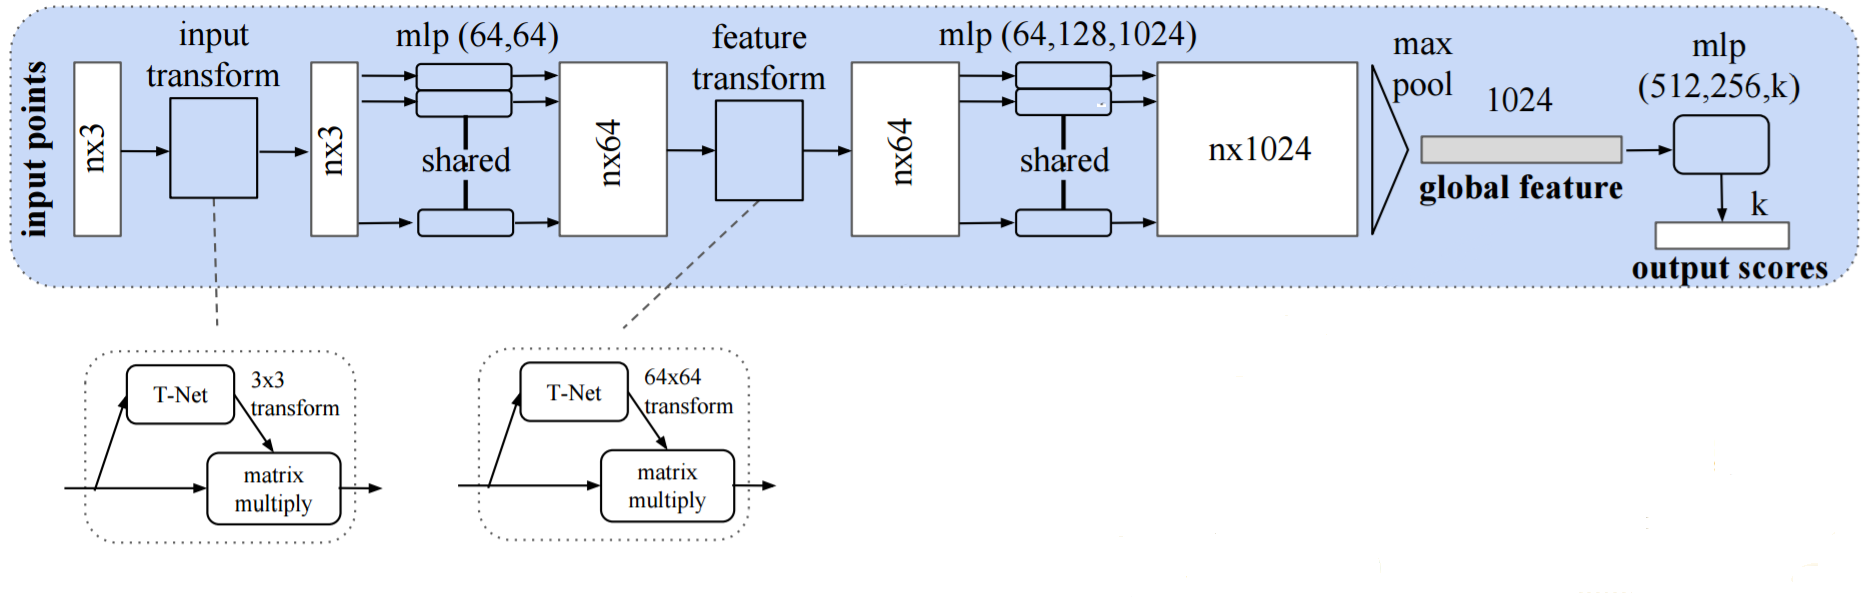
\includegraphics[scale=0.3]{classification_network}
    \end{figure}  
  \end{frame}
  
  \begin{frame}
    \frametitle{Problems}
    
    Problems when predicting point sets:
    \begin{itemize}
      \item How to appropriately compare two unordered point sets?
      \item How to model uncertainty?
    \end{itemize}
  \end{frame}
  
  \begin{frame}
    \frametitle{Comparing Point Sets}
    Chamfer Distance (CD) for point sets $X = \{x_1, \ldots,x_n\}$, $Y = \{y_1,\ldots,y_m\}$:
    \begin{align}
      d_{\text{CD}}(X, Y) = \sum_{x \in X} \min_{y \in Y} \|x - y\|_2^2 + \sum_{y \in Y}\min_{x \in X} \|x - y\|_2^2.\notag
    \end{align}    
    Easily implemented (and parallelizable).
  \end{frame}
  
  \begin{frame}
    \frametitle{Comparing Point Sets (cont'd)}
    Earth Mover Distance (EMD) for point sets $X$, $Y$ with $|X| = |Y|$:
    \begin{align}
      d_{\text{EMD}} = \min_{\phi:X \mapsto Y} \sum_{x \in X} \|x-\phi(x)\|_2\notag
    \end{align}
    with $\phi$ being a bijection.
    \vskip 1em
    
    Exact computation not feasible; $(1 + \epsilon)$ approximation \cite{Bertsekas:1985} used.
  \end{frame}
  
  \begin{frame}
    \frametitle{Model Uncertainty}
    Possibilities:
    \begin{itemize}
      \item (Conditional) generative adversarial networks \cite{Goodfellow:2014,MirzaOsindero:2014};
      \item (Conditional) variational auto-encoders \cite{KingmaWelling:2013,KingmaMohamedRezendeWelling:2014,SohnLeeYan:2015}.
    \end{itemize}
    \vskip 1em
  \end{frame}
  
  \begin{frame}
    \frametitle{Model Uncertainty (cont'd)}
    Inject randomness as additional input (i.e. noise vector): $G(I, \epsilon)$.
    \vskip 1em
    Minimize
    \begin{align}
      \sum_k \min_{\epsilon_j \in \mathcal{N}(0, 1)} d(G(I_k, \epsilon_j), S_k)\notag
    \end{align}
    for $j \in \{0,\ldots,n\}$, $I_k$ being the input image and $S_k$ the ground truth point set.
    \vskip 1em
    So-called ``Min-of-N'' loss.
  \end{frame}
  
  \begin{frame}
    \frametitle{Network Architecture}
    \begin{figure}
      \centering
      \hspace*{-0.5cm}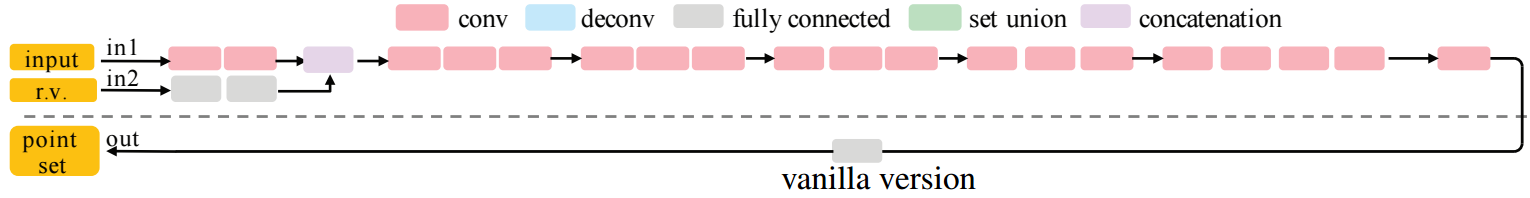
\includegraphics[scale=0.29]{architecture_1}
    \end{figure}
  \end{frame}
  
  \begin{frame}
    \frametitle{Network Architecture (cont'd)}
    \begin{figure}
      \centering
      \hspace*{-0.5cm}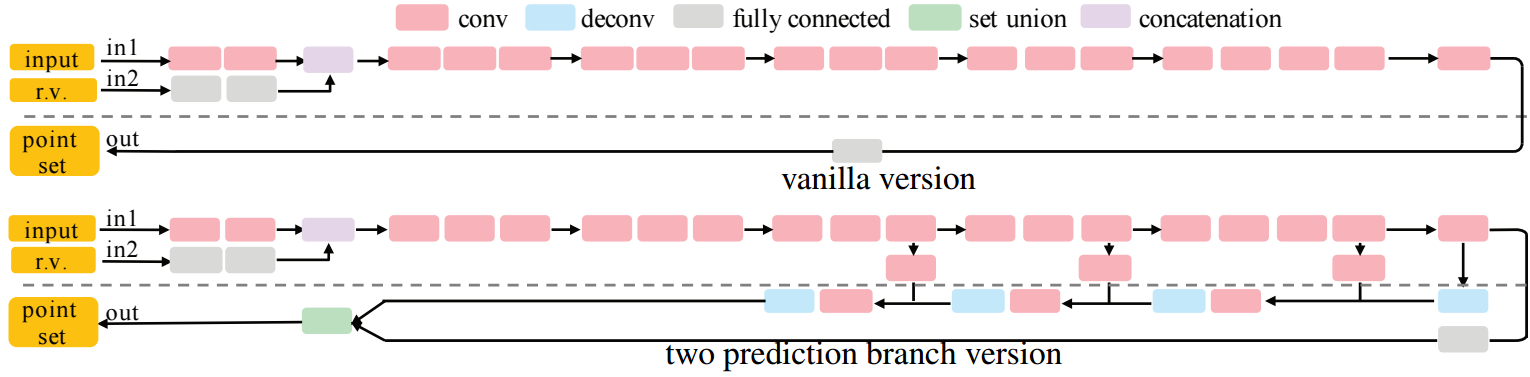
\includegraphics[scale=0.29]{architecture_2}
    \end{figure}
  \end{frame}
  
  \begin{frame}
    \frametitle{Network Architecture (cont'd)}
    \begin{figure}
      \centering
      \hspace*{-0.5cm}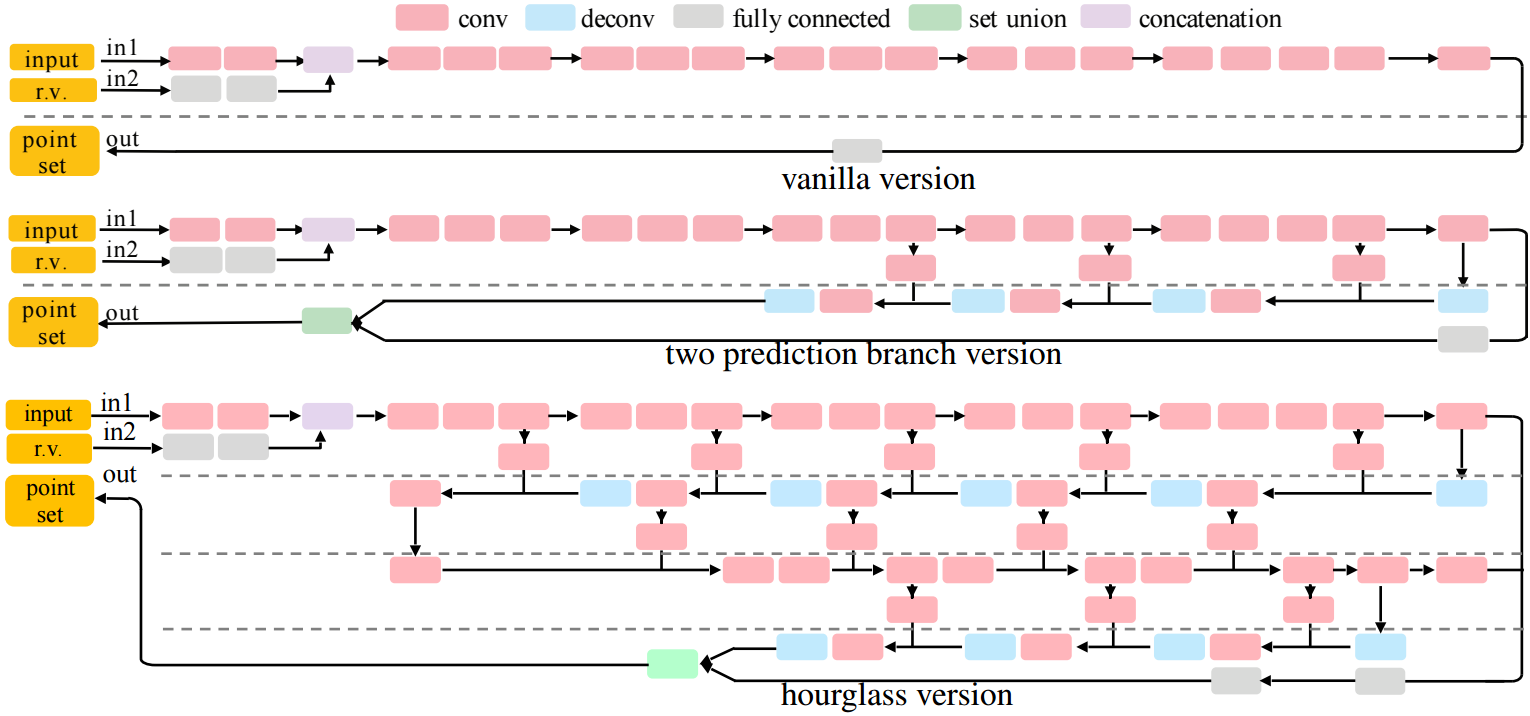
\includegraphics[scale=0.29]{architecture}
    \end{figure}
  \end{frame}
  
  \begin{frame}
    \frametitle{3D Reconstruction (RGB)}
    Experimental Setup:
    \begin{itemize}
      \item rendered models (RGBD) from ShapeNet \cite{Chang:2015};
      \item unclear how many points are predicted -- for two-branch: 256 + 768 points;
      \item unclear how the ground truth point sets are chosen;
      \item evaluation using Intersection-over-Union (IoU) on voxels.
    \end{itemize}
  \end{frame}
  
  \begin{frame}
    \frametitle{3D Reconstruction (RGB) (cont'd)}
    \begin{table}
      \begin{tabular}{l | c}
        & Mean IoU\\\hline
        3D-R2N2 \cite{Choy:2016} 1 views & 0.560\\
        3D-R2N2 \cite{Choy:2016} 3 views & 0.617\\
        3D-R2N2 \cite{Choy:2016} 5 views & 0.631\\
        PointNet & 0.64
      \end{tabular}
      \caption{Intersection-over-Union results on ShapeNet \cite{Chang:2015} compared to 3D-R2N2 \cite{Choy:2016}.}
    \end{table}
  \end{frame}
  
  \begin{frame}
    \frametitle{3D Reconstruction (RGB) (cont'd)}
    \begin{figure}
      \begin{subfigure}[t]{0.18\textwidth}
        \centering
        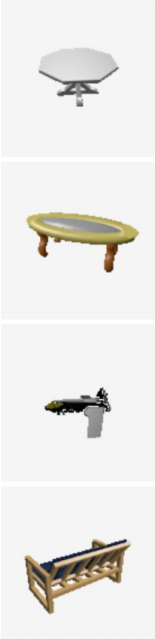
\includegraphics[scale=0.39]{qual_rgb_input}\\
        {\footnotesize input}
      \end{subfigure}
      \begin{subfigure}[t]{0.18\textwidth}
        \centering
        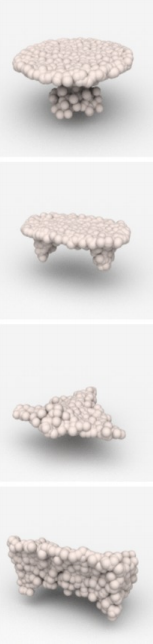
\includegraphics[scale=0.39]{qual_rgb_output}\\
        {\footnotesize output}
      \end{subfigure}
      \begin{subfigure}[t]{0.18\textwidth}
        \centering
        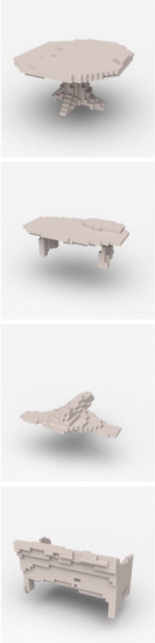
\includegraphics[scale=0.39]{qual_rgb_post}\\
        {\footnotesize post-\\[-4px]processed}
      \end{subfigure}
      \begin{subfigure}[t]{0.18\textwidth}
        \centering
        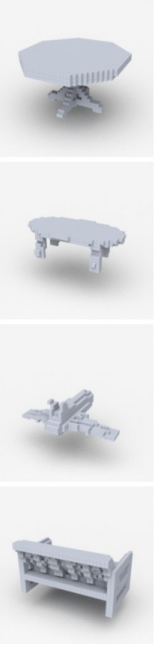
\includegraphics[scale=0.39]{qual_rgb_gt}\\
        {\footnotesize ground\\[-4px]truth}
      \end{subfigure}
      \begin{subfigure}[t]{0.18\textwidth}
        \centering
        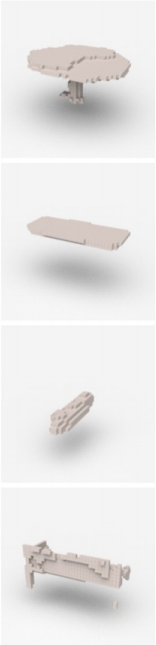
\includegraphics[scale=0.39]{qual_rgb_3d}\\
        {\footnotesize 3D-R2N2 \cite{Choy:2016}}
      \end{subfigure}
    \end{figure}
  \end{frame}
  
  \begin{frame}
    \frametitle{3D Shape Completion (RGBD)}
    
    \begin{figure}
      \centering
      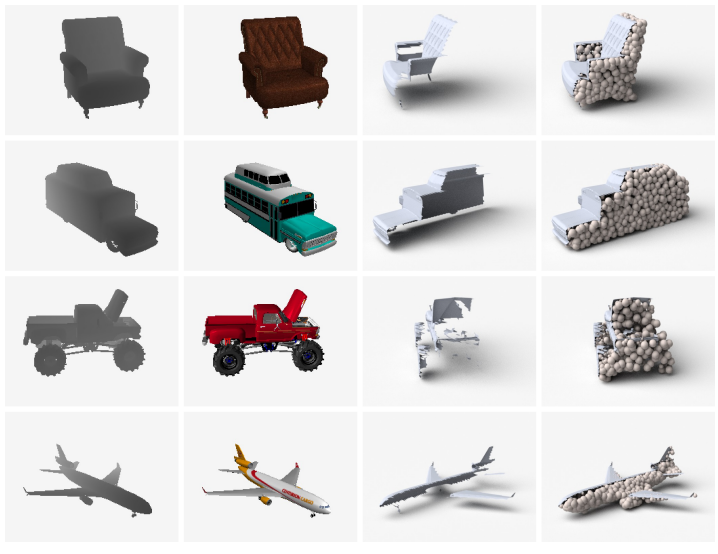
\includegraphics[scale=0.5]{shape_completion}
    \end{figure}
  \end{frame}
  
  \begin{frame}
    \frametitle{Deconvolution vs. Fully Connected}
    \begin{figure}
      \centering
      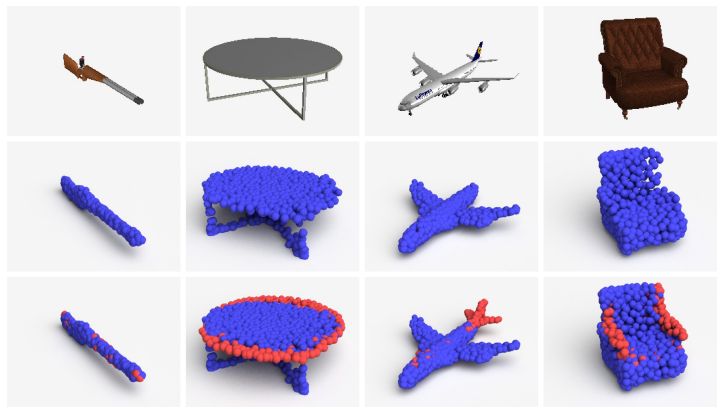
\includegraphics[scale=0.5]{deconv}
    \end{figure}
  \end{frame}
  
  \begin{frame}
    \frametitle{My 2 Cents ...}
    Some experiments missing:
    \begin{itemize}
      \item Quantitative comparison of (C)VAE or (C)GAN with MoN loss;
      \item comparison of vanilla, two branches and hourglass with respect to IoU.
    \end{itemize}
  \end{frame}
  
  \begin{frame}
    \frametitle{Conclusion}
    3D reconstruction by using a CNN to predict a set of points -- trained on synthetic data.
    \vskip 1em
    
    Interesting in combination with PointNet, allows to directly operate on and predict unordered sets of points.
    \begin{itemize}
      \item The only two works on deep learning on 3D point sets ...
    \end{itemize}
  \end{frame}
  
  \begin{appendix}
    \begin{frame}
      \frametitle{Distances}
      \begin{figure}
        \centering
        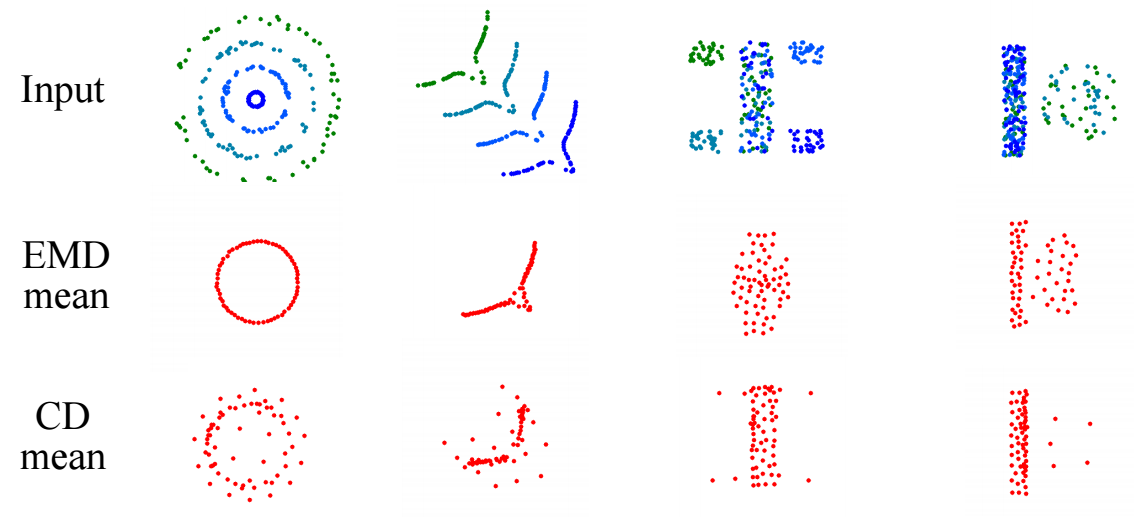
\includegraphics[scale=0.35]{cd_emd}
      \end{figure}
    \end{frame}
    
    \begin{frame}
      \frametitle{VAE Comparison}
      \begin{figure}
        \centering
        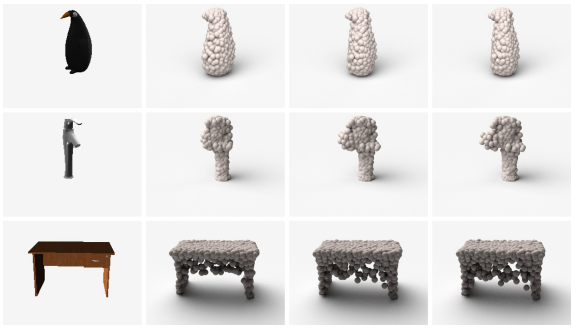
\includegraphics[scale=0.65]{multiple_mon}
        \caption{Multiple predictions using the MoN loss.}
      \end{figure}
    \end{frame}
    
    \begin{frame}
      \frametitle{VAE Comparison (cont'd)}
      \begin{figure}
        \centering
        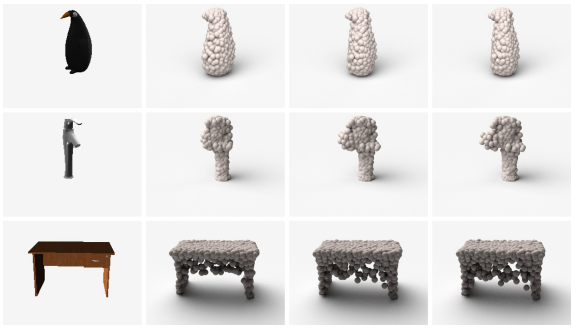
\includegraphics[scale=0.65]{multiple_mon}
        \caption{Multiple predictions using a (C)VAE formulation.}
      \end{figure}
    \end{frame}
    
    \begin{frame}
      \frametitle{Real Examples}
      \begin{figure}
        \centering
        \hspace*{-0.25cm}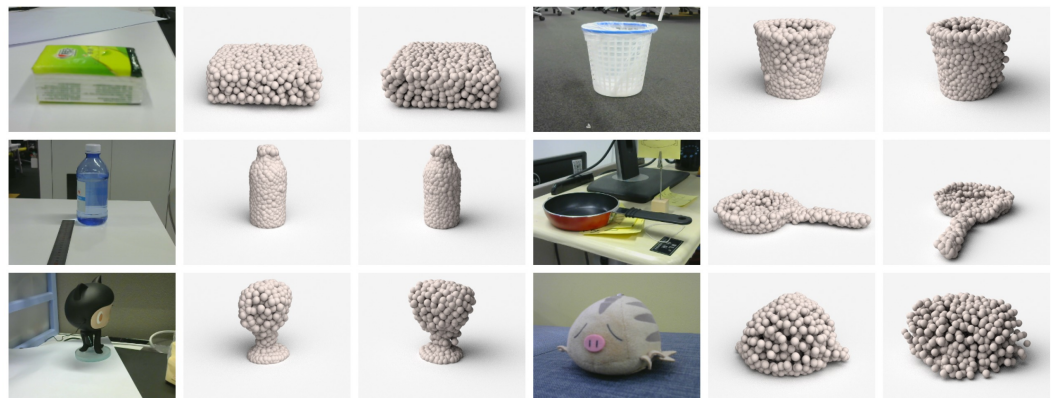
\includegraphics[scale=0.4]{real}
        \caption{Multiple predictions on real examples; objects were masked out.}
      \end{figure}
    \end{frame}
  \end{appendix}
  
  \begin{frame}[allowframebreaks]
    \frametitle{References}
    \bibliography{slides} 
    \bibliographystyle{plain}
  \end{frame}
\end{document}
